\documentclass[12pt]{article}
\usepackage{epsfig,a4}
%\usepackage{draftcopy}
\begin{document}
\thispagestyle{empty}
\title{CloudMan: design document Update 4}
\author{CERN IT-DEP/PES-PS}
%\version{0.0.1}
\date{\today}
\maketitle 
\begin{abstract}
This document describes the design for the Betelgeuze release of CloudMan.
\end{abstract}
%
% contents
%
\tableofcontents
\listoffigures 

%
% introduction 
%
\section{Purpose of this document} 
Concepts and initial ideas of the CloudMan project are described in~\cite{CloudManProject}. The purpose of this document is to define interfaces and the design of the modules, aiming at the implementation of the tool. An overview over the architecture is given in fig.~\ref{architecture}, as described in ~\cite{CloudManProject}.

As a general guideline, standard OpenSource tools and frameworks, and/or existing services should be used where ever possible. 

\begin{figure}
\begin{center}
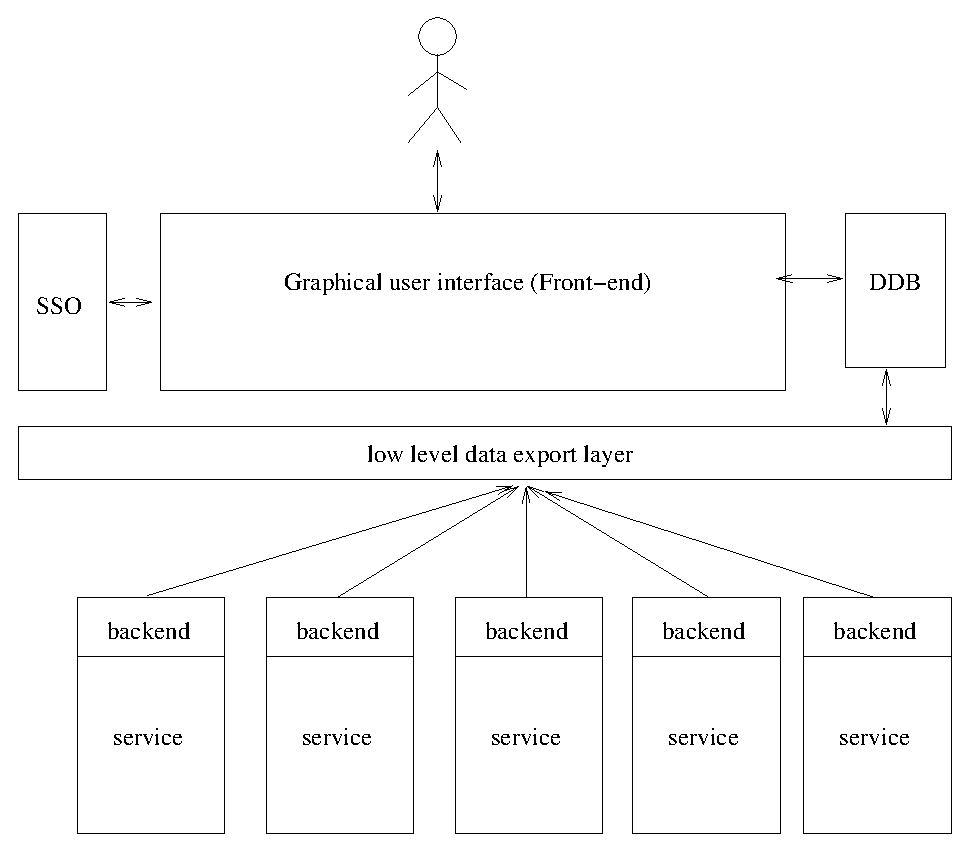
\includegraphics[width=0.9\textwidth]{architecture2.eps}
\caption{\label{architecture} Basic architecture of the desired system. Users connect to the front-end which offers a graphical user interface. They authenticate using the site Single Sign On mechanism or similar. The data which is entered is stored in an external database, and exported in a low level format. Back-ends which are design to configure specific services, for example local cloud installations, consume this information to configure their resources.}
\end{center}
\end{figure}



%
% goals of phase 1
%
\section{First phase implementation goals}
The aim of first phase of the project is the implementation of 
\begin{itemize}
\item The graphical user interface 
\begin{itemize}
  \item the GUI itself is stateless
  \item all data is kept in a database backend (mysql,oracle)
  \item the GUI is accessible behind a (load balanced or round robin) alias. For example, at CERN one instance can be run at Meyrin, the second at SafeHost, thus providing redundancy.
  \item the application should be implemented in Django\cite{Django} framework, running on an Apache web server with Shibboleth for implemeting SingleSignOn   
  \item access is secured via SSL. For the CERN instance, CERN will provide a certificate signed by the CERN CA.
  \item Low-level data export is visible inside CERN without any Authentication.
\end{itemize}
\item The database backend
\begin{itemize}
  \item Oracle is preferred, as it is supported at CERN, and provides fail-over mechanisms. 
  \item the database access should be abstracted using the Django Object Relational Model (ORM)\cite{ORM}; writing direct SQL statements should be avoided \footnote{MySQL or similar (eg SQLite) can be used during development}
  \item the backend database should have transaction support to insure data integrity when doing multiple updatesDjango Object Relational Model (ORM)\cite{ORM} transaction support can be used.
\end{itemize}
\item Authentication
\begin{itemize}
\item It must be possible to use CERN SSO~\cite{CernSSO} to authenticate users. The CERN instance will only use this mechanism for authentication
\item Access will stay in SSL secured after login
\end{itemize}
\item Authorization
\begin{itemize}
\item Users can belong to one or more VOs, and can have different roles inside these VOs. The VO membership is determined by the Unix group IDs of the person which is retrieved from LDAP.
\item multiple VO memberships are mapped to multiple (secondary) Unix group IDs 
\item There is one and only one resource manager role. The list of these users is retrieved from LDAP. The unix group ID of these users is irrelevant.
\item Ordinary users only have access to information which belongs to the VO(s) they belong to, determined by their unix group IDs
\item The role of a user inside his VO is determined by the egroups~\cite{CernEgroups} he belongs to
\item the use of egroups~\cite{CernEgroups} allows to move much of the complexity due to the hierarchi of roles into this existing service.
\item the egroups used for mapping users to roles must be configurable via the GUI, respecting ACLs and hierarchies
\item in case egroups is not available (eg outside CERN), simple lists of users can be supported as well but are discouraged.  
\end{itemize}
\item data export level
\begin{itemize}
\item the backends will pull the information required to configure themselves from the low level data export layer which is fed by the GUI. 
\item in the second project phase the backend will report back on the  current resource consumption which can be polled by the GUI. The data exchange model is identical.
\item if the exported data contains fields which are not supported by a backend, the backend can ignore this data
\item if Django is used, each backend will be served by a distinct URL providing only the information required for this specific backend
\item the data export is done in a machine readable way, eg via a XML,JSON,yaml format. 
\item the data export is SSL secured 
\item in the first phase of the project a check of the authentication of the backends is not required. This will change in the second phase, when the authenticity of the reported data by the backends has to be checked
\item all changes done in the front end must be traceable, including information about 
\begin{itemize}
 \item what has been changed 
 \item what operation has been done 
 \item when it has been changed
 \item who applied the change
\end{itemize}
\end{itemize}
\item backends which are part of the project
\begin{itemize}
\item a sample backend to configure OpenStack
\item a sample backend to configure OpenNebula
\item a sample backend to configure batch resources 
\item a sample backend to configure CASTOR 
\end{itemize}
\end{itemize}
All backends must support a no-action mode, as well as different logging levels (info, error, debug), ideally through syslog.


%
% Use cases
%
\section{Use cases}
CloudMan will be used to manage an IaaS based computer center layout, as shown in figure~\ref{iaas}. The use cases naturally derive from this model. In this picture, each application comes with a backend which uses information from CloudMan to configure itself, respecting the allocations of resources to each defined user community.
\begin{figure}
\begin{center}
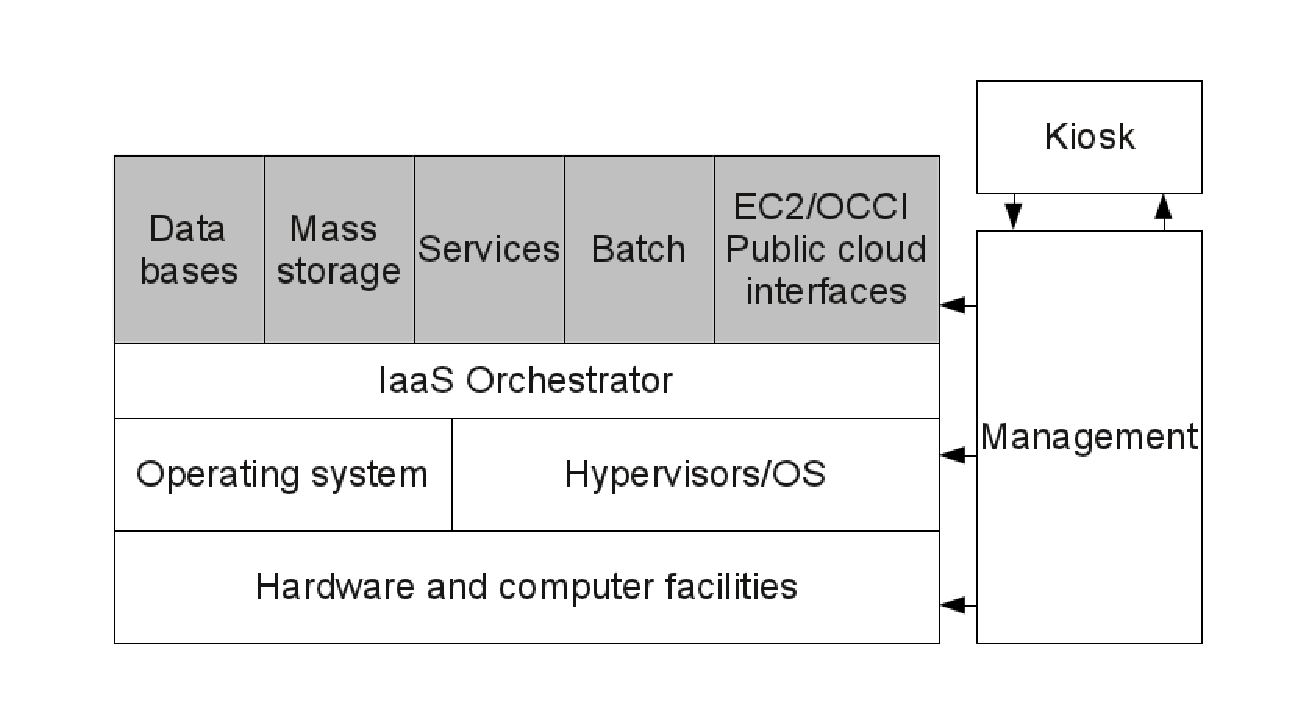
\includegraphics[width=\textwidth]{iaas.eps}
\caption{\label{iaas}Vision of a high level structure for an IaaS based computer center. CloudMan will be an essential part of the management layer for this model.}
\end{center}
\end{figure}
CloudMan must be capable to cope with the configuration of the use cases:
\begin{itemize}
\item Global allocations for individual IT services like 
\begin{itemize}
\item lxbatch resources, physical and virtual~\footnote{These correspond to different resource pools} 
\item public cloud resources for general use
\item storage resource pools for CASTOR and SWIFT
\item storage resource pools for virtual batch scratch and AFS cache space
\item physical resource pools for databases
\end{itemize}
\item The configuration of quotas per VO for an EC2 based self-service
\item The enforcement of quotas for reliable resources, based on total resources per VO by the resource manager
\item The configuration of shares for the batch farm VO project admins and subproject admins
\begin{itemize}
 \item The total resource allocation, typically in kSi2K for shared batch resources is done directly by the resource manager 
 \item The resource manager only defines a global allocation for each VO for resource pools used by the batch farm
 \item The difference between allocations done for the VOs and totally available resources for lxbatch are used for a public share
 \item The VO responsibles for projects and subprojects decide for which applications these resources are used. The fraction of resources allocated to batch processing is translated by the corresponding backend into a fair share value.
\end{itemize}
\end{itemize}

The following specific use cases are identified:
\begin{itemize}
\item new CPU resource have arrived for use by the self service
\item the fraction of SLC5 and SLC6 resources in lxbatch needs to be changed 

\end{itemize}



%
% details
%
\section{Details}
\section{Details}
This section describes the details necessary for the implementation of the different modules.

\begin{figure}
\begin{center}
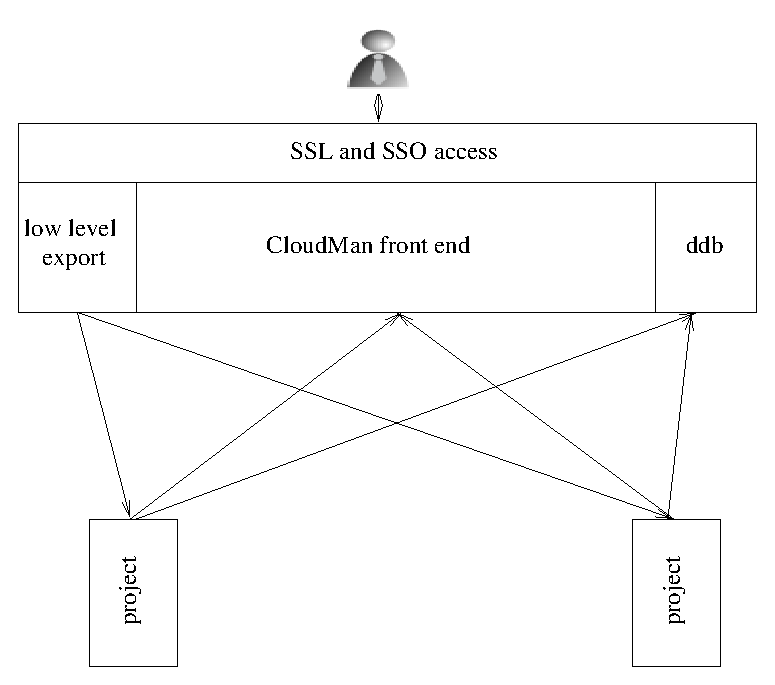
\includegraphics[width=0.9\textwidth]{cloudman_highlevel.eps}
\caption{\label{architecture} Updated architecture of the desired system. Users connect to the front-end which offers a graphical user interface. The side is secured with SSL techniques. All users have to authenticate using the sites Single Sign On mechanism. The data which is entered is stored in an external database and exported in a low level format. Shown in this figure are project specific backends only. In general these backends are site specific, and design to configure specific services. Each backend reads the data which it needs to configure it's resources from the low level export layer from CloudMan. The current state which includes error or warning conditions is reported back to the frontend as well as the CloudMan database. The database is used to record the historical state data per project backend.}
\end{center}
\end{figure}
Fig.~\ref{architecture} shows an overview over the CloudMan architecture. Users have to authenticate using SSO. After login, the communication stays secured by SSL. Project backends report their state asynchronously via a file or URL. The state data is recorded in the database to save the history. 


\subsection{Definition of Interfaces}
\subsubsection{CloudMan database schema}
An SQL database is used for the backend database. 

The following information is required:
\begin{itemize}
\item Super User name or e-group
\item Resource definitions and units
\item Resource features 
\item Roles
\item Map of user names or e-groups to roles
\item Table with historical state data for all project backends
\end{itemize}

The database holds all dynamic information. Static configuration data goes into the configuration files, see there. 
Certain information like the meta data of resource pools may change during the lifetime of the product. The database schema is made in such a way that it is easy to add or remove features which were not there at the beginning to the schema without having to perform complicated and slow database operations. 

\begin{figure}
\begin{center}
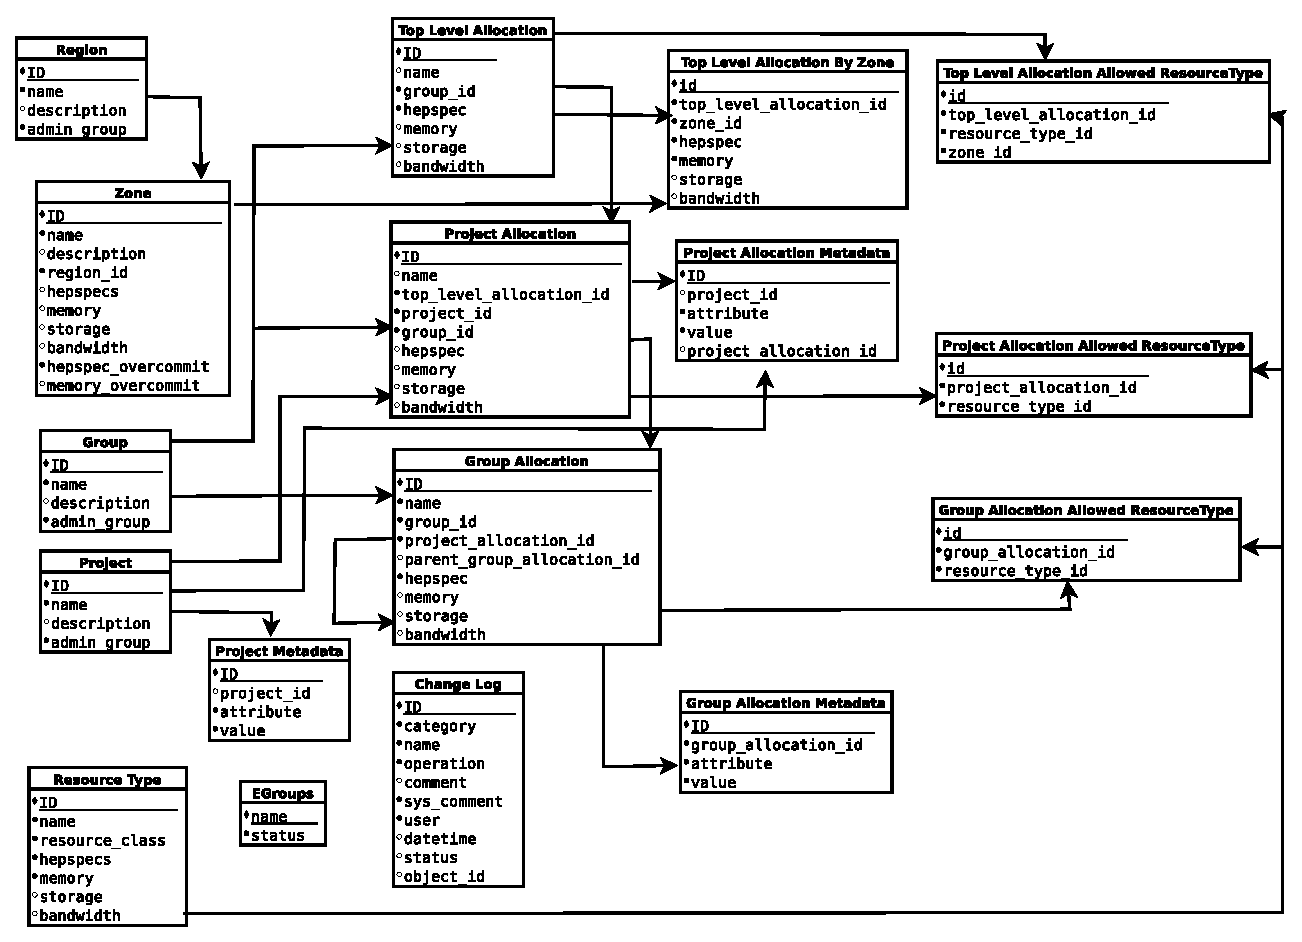
\includegraphics[width=\textwidth]{cloudman_db.eps}
\caption{\label{ddb_schema_new} Cloudman database schema, Betelgeuze release.}
\end{center}
\end{figure}

The figure ~\ref{ddb_schema_new} shows the final database schema for the FIXME:Aldebaran release of CloudMan.


The description of resources is kept in the database as well. This way, it is easy to define new valid resource attributes directly via the web interface. Updating this table is reserved to the resource manager role who owns all privileges. 

Resources and groups are matched at the top level by the resource manager in the process of filling in the allocations. Allocations are done in terms of CPU, disk and memory for each resource available. 
The resource manager approves requests for the allocations. Only approved allocations will be exported, 
and used by the back-ends.

At the lower levels, the managers do allocations out of the quota which have been allocated to them by an upper instance. 





\subsubsection{Low level data export layer}
The low level data export layer publishes the configuration data entered in the front end, so that it can be consumed by the different backends.
The data and the format should be customizable for each backend. 
This can be done for example by exploiting features of Django.  

In the second phase of the project, the same mechanism shall be used by the backends to provide live monitoring information about their current status.




\subsubsection{Configuration files}
Static configuration data can be stored in configuration files on the 
server(s) but should be avoided, in order to keep the service stateless. 
Instead, such configuration data should be entered in the GUI and 
stored in the database. 

In case such a file is needed anyway, the format must be plain text, 
so that it can be easily manipulated by configuration components
 eg from Quattor (or Puppet). The development of such 
components is NOT part of this project. The format must be key-value pairs, 
following the python config parser format {\it FIXME: add reference}
 
 




\section{Resource pools}
Resource pools in CloudMan only have high level meta data information, like
\begin{itemize}
\item identifier (eg like landb cluster name)
\item description
\item size 
\item type
\item features 
 \begin{itemize}
 \item public or not
 \item support for life migration or not
 \item reliable or not, critical power etc 
 \item GPN/LCG network
 \item {\it what else }
 \end{itemize}
\end{itemize}
There are mandatory and optional fields. 
It must be easy to add additional fields without having to 
change the application.
 



\section{Backends}
Backends are plugins to CloudMan which can and should be shipped separately from the CloudMan interface itself. This way it is easy to deploy highly customized backends which consume the data from the central interface. The base distribution 
of CloudMan can therefore ship with a sample implementation for such a backend. 

Possible backends include 
\begin{itemize}
\item One or more plugins to configure batch system shares, one per batch system in use (eg LSF, SLURM, ...)
\item One or more plugins to configure an OpenNebula instance
\item One or more plugins to configure an OpenStack instance
\end{itemize}
Plugins are expected to be project driven but they don't have to be. This is specifically true for plugins which talk to
an internal cloud setup: A site may choose to have one plugin for each tenant in an OpenStack instance, or rather use
only one plugin which will configure the whole cloud instance. 

\subsection{Batch shares}
CloudMan should support the definition of shares for a batch processing project. 
Such a backend is particularly interesting for CERN because there is already an
existing application ({\it LSFweb}) which has been designed before SSO and 
egroups were introduced at CERN. The new backend will allow to replace this old 
tool. 

When determining resources for a batch farm, there are two aspects which need
to be considered:

\begin{enumerate}
\item the batch processing resources: The batch farm itself has a certain size, that is a number of worker nodes providing job slots, which are available for the users to process their data. In the simplest case all worker nodes are organized in a single public partition which can be accessed by all registered users. At CERN, the situation is more complicated though. Although all CPU resources belong to the same batch instances, there are additional partitions providing dedicated resources to some user groups. 
The bulk of computing resources at CERN consist of physical worker nodes. The configuration of these resources is currently done using the Quattor tool kit. At the long term there are plans to virtualize more and more of these resources, and provide them through an internal cloud. It should be possible to use CloudMan to manage such resources, for example through a batch resource project. 
 
\item the user shares: Some of the batch partitions implement fair share. At CERN, batch shares are currently managed through a graphical user interface called
LSFweb. It should be possible to manage LSF shares through a batch project from CloudMan, allowing to replace the old LSFweb tool.
\end{enumerate}

CloudMan shall offer a way to configure both batch resources and batch user shares from a single interface. 

The goal for the first design phase is to develop a prototype of a backend for the second use cases. Ideally, some tools should be provided which allow to migrate from LSFweb to CloudMan in an easy way.

\subsection{OpenNebula}
%The OpenNebula backend is meant mainly as a playground until an OpenStack testbed is available. 
With the availability of an OpenStack testbed the priority of developing a backend for OpenNebula has dropped for CERN. The OpenNebula based infrastructure at CERN is planned to be retired at end 2012 or early 2013, and absorbed in the new OpenStack based infrastructure. Therefore the priority is moved to OpenStack. 



\subsection{OpenStack}
The planned OpenStack backend can be derived from the OpenNebula backend. Projects will be mapped to tendants. 
As in the OpenNebula case, the backend will create a new tenant for each leaf in the tree defined in CloudMan.

Thus, the OpenStack backend relies on the possibility to set quotas per tenant. 
 



\section{Benefits, assumptions, risks/issues}
Writing backends for Cloud controllers like OpenStack and Opennebula bears some risk as the concepts and definitions used by those young projects are still changing rapidly. In addition, the backends for these systems will be very model dependent, in the sense that each site who deploys them will configure them differently. 

 

%
% references
%
\begin{thebibliography}{99}
%
% references
%
\bibitem{ORM}
http://en.wikipedia.org/wiki/Object-relational\_mapping
\bibitem{Django}
https://www.djangoproject.com
\bibitem{CloudManProject}
CloudMan: project description, CERN IT-DEP/PES-PS, July 2011
\bibitem{CernSSO}
https://espace.cern.ch/authentication/CERN\%20Authentication\%20Help/Integrate\%20CERN\%20SSO\%20in\%20Apache.aspx
\bibitem{CernEgroups}
https://espace.cern.ch/e-groups-help/default.aspx
\bibitem{ONE}
See: http://opennebula.org
\bibitem{OPENSTACK}
See: http://opensstack.org
%\bibitem{LSF}
%Release Notes for Platform LSF Version 7.0, Nov. 2006,  PLATFORM corporation.
\bibitem{XEN}
http://www.xen.org
\bibitem{KVM}
http://www.linux-kvm.org
\bibitem{arne}
priv. comm. Arne Wiebalck, CERN-IT
\bibitem{luca}
priv. comm. Luca Mascetti, CERN-IT

\end{thebibliography}
\end{document}


